\documentclass[letterpaper,11pt,twoside]{article}
\usepackage[margin=0.88in]{geometry}

%%%%%%%%%%%%%%%%%%%%%%%%%%%%%%%%%%%%%%%%%%%%%%%%%%%%%%%%%%%%%%%%%%%%%%%%%%%%%%%


\def\mypdfauthor{Dimitris Diochnos}
\def\mypdfsubject{Undergraduate Course}
\def\mypdftitle{CS 3823 - Theory of Computation, 2025F: HW2}
\def\myheadertitle{CS 3823 - Theory of Computation: Homework Assignment 2}
\def\mytitle{CS 3823 - Theory of Computation: Homework Assignment 2}
\def\thecurrentsemester{Fall 2025}
\def\myduedate{\textbf{Due:} Friday, October 3, 2025}


%%%%%%%%%%%%%%%%%%%%%%%%%%%%%%%%%%%%%%%%%%%%%%%%%%%%%%%%%%%%%%%%%%%%%%%%%%%%%%%


\usepackage{xspace}
\usepackage{enumitem}
%\usepackage[numbers,square,sectionbib,sort&compress]{natbib}
\usepackage[numbers,square,sort&compress]{natbib}
\usepackage[euler-digits, T1]{eulervm}
\usepackage{upgreek}
\usepackage[dvipsnames]{xcolor}
\usepackage[
   colorlinks%
   ,plainpages=false%This forces a unique identification of pages.
   ,hypertexnames=true%This is necessary to have exact link on Index page.
   ,naturalnames
   ,hyperindex
   ,citecolor=OliveGreen
   ,urlcolor=RoyalBlue
   ,pdfauthor={\mypdfauthor}
   ,pdftitle={\mypdftitle}
   ,pdfsubject={\mypdfsubject}
   %,pdfkeywords={...}
]{hyperref}
%\usepackage{lettrine}
%\input{definitions}
\usepackage{psfrag}
\usepackage{graphicx}
\usepackage{multirow}
\usepackage{multicol}
%\usepackage{vwcol}
\usepackage{enumitem}

%%%%%%%%%%%%%%%%%%%%%%%%%%%%%%%%%%%%%%%%%%%%%%%%%%%%%%%%%%%%%%%%%%%

\usepackage{bm}
\usepackage{pstricks}
\psset{unit=0.45cm}
\psset{linewidth=0.05}%
\psset{fillstyle=solid}%

\newcommand{\sample}{\ensuremath{S}\xspace}
\newcommand{\XX}{\ensuremath{\mathcal{X}}\xspace} % X

%%%%%%%%%%%%%%%%%%%%%%%%%%%%%%%%%%%%%%%%%%%%%%%%%%%%%%%%%%%%%%%%%%%

\usepackage{fancyhdr}
\pagestyle{fancy}
\usepackage{lastpage}

\setlength{\headheight}{14pt}

\fancypagestyle{firststyle}
{
   \fancyhf{}
   \fancyfoot[L]{\today}
   %\fancyfoot[C]{\thepage/\pageref*{LastPage}}
   \fancyfoot[R]{\thepage/\pageref*{LastPage}}
}


\newcommand{\stylishPagesColor}{Gray}
\newcommand{\stylishHref}[2]%
{\hypersetup{urlcolor=\stylishPagesColor}%
\href{#1}{#2}%
\hypersetup{urlcolor=RoyalBlue}}


\fancyhead{} % clear all header fields
\fancyhead[CO,CE]{\textsc{\myheadertitle}}
\fancyfoot{} % clear all footer fields
\fancyfoot[LO,RE]{\today}
\fancyfoot[RO,LE]{\thepage/\pageref*{LastPage}}
\renewcommand{\headrulewidth}{0.0pt}
\renewcommand{\footrulewidth}{0.0pt}
%%%%%%%%%%%%%%%%%%%%%%%%%%%%%%%%%%%%%%%%%%%%%%%%%%%%%%%%%%%%%%%%%%%
\newcommand{\OO}[1]{\ensuremath{\mathcal O\left(#1\right)}\xspace}
\newcommand{\OOs}[1]{\ensuremath{\widetilde{\mathcal O}\left(#1\right)}\xspace}
%%%%%%%%%%%%%%%%%%%%%%%%%%%%%%%%%%%%%%%%%%%%%%%%%%%%%%%%%%%%%%%%%%%
% So that absolute values and norms are neat.
\usepackage{amsmath}
\providecommand{\abs}[1]{\lvert#1\rvert}
\providecommand{\norm}[1]{\lVert#1\rVert}
% Sets
\providecommand{\set}[1]{\ensuremath{\left\{#1\right\}}\xspace}
\providecommand{\powerset}[1]{\ensuremath{\mathcal{P}\left( #1\right)}\xspace}

%%%%%%%%%%%%%%%%%%%%%%%%%%%%%%%%%%%%%%%%%%%%%%%%%%%%%%%%%%%%%%%%%%%
\providecommand{\emptystring}{\ensuremath{\varepsilon}\xspace}
\newcommand{\emptysymbol}{\varepsilon}
\newcommand{\regexpunion}{\ensuremath{\cup}\xspace}
%%%%%%%%%%%%%%%%%%%%%%%%%%%%%%%%%%%%%%%%%%%%%%%%%%%%%%%%%%%%%%%%%%%

\usepackage{color}
\definecolor{RoyalBlue}{cmyk}{1, 0.50, 0, 0}
\definecolor{ForestGreen}{cmyk}{0.864, 0.0, 0.429, 0.396}
\definecolor{Brown}{cmyk}{0.0,0.692,0.925,0.529}

\newcommand{\WriteRoyalBlue}[1]{{\color{RoyalBlue} #1 }\xspace}
\newcommand{\WriteForestGreen}[1]{{\color{ForestGreen} #1 }\xspace}
\newcommand{\WriteBrown}[1]{{\color{Brown} #1 }\xspace}
\newcommand{\WriteCustomColor}[1]{{\color{blue} #1 }\xspace}
\newcommand{\WriteSolutions}[1]{\WriteCustomColor{#1}}

%%%%%%%%%%%%%%%%%%%%%%%%%%%%%%%%%%%%%%%%%%%%%%%%%%%%%%%%%%%%%%%%%%%

\newcommand{\us}{\selectlanguage{american}}
\newcommand{\gr}{\selectlanguage{greek}}

%%%%%%%%%%%%%%%%%%%%%%%%%%%%%%%%%%%%%%%%%%%%%%%%%%%%%%%%%%%%%%%%%%%




\begin{document}

%%%%%%%%%%%%%%%%%%%%%%%%%%%%%%%%%%%%%%%%%%%%%%%%%%

\author{
\textsc{\thecurrentsemester} \hspace{3cm}\myduedate
}
\title{\mytitle}
\date{}
\maketitle

%%%%%%%%%%%%%%%%%%%%%%%%%%%%%%%%%%%%%%%%%%%%%%%%%%

\thispagestyle{firststyle}

%%%%%%%%%%%%%%%%%%%%%%%%%%%%%%%%%%%%%%%%%%%%%%%%%%

\vspace{-0.5cm}
\noindent\makebox[\linewidth]{\rule{\columnwidth}{2pt}}

% Linz's book:
%\noindent\textbf{Related Reading.} Sections 2.1, 2.2, 2.3, 3.1, 3.2, 4.1\\
% Sipser's book:
\noindent\textbf{Related Reading.} Chapter 1\\
\noindent\textbf{Instructions.} Near the top of the first page of your solutions please list clearly \textbf{all} the members of the group (\underline{please see the syllabus for the collaboration policy}) who have created the solutions that you are submitting. Listing the names of the people in the group implies their full name and their 4x4 IDs.
Alternatively, you can use the space below and provide the relevant information 
in case you submit the solutions using this document.\\ 
\noindent\makebox[\linewidth]{\rule{\columnwidth}{2pt}}


\begin{center}
\textbf{Student Information for the Solutions Submitted}
\end{center}

\begin{center}
\begin{tabular}{c|c|c|}\cline{2-3}
 & Lastname, Firstname
 & 4x4 ID (e.g., dioc0000)
 \\\hline
%\multicolumn{1}{|c|}{\multirow{2}{*}{\textbf{1}}}
\multicolumn{1}{|c|}{\multirow{2}{*}{1}}
& \phantom{ABCDEFGHIJKLMNOPQRSTUVWXYZ0123456789} & \phantom{dioc0000dioc0000} \\
\multicolumn{1}{|c|}{}
           & \phantom{ABCDEFGHIJKLMNOPQRSTUVWXYZ0123456789} & \phantom{dioc0000dioc0000} \\\hline
%\multicolumn{1}{|c|}{\multirow{2}{*}{\textbf{2}}}
\multicolumn{1}{|c|}{\multirow{2}{*}{2}}
& \phantom{ABCDEFGHIJKLMNOPQRSTUVWXYZ0123456789} & \phantom{dioc0000dioc0000} \\
\multicolumn{1}{|c|}{}
           & \phantom{ABCDEFGHIJKLMNOPQRSTUVWXYZ0123456789} & \phantom{dioc0000dioc0000} \\\hline
%\multicolumn{1}{|c|}{\multirow{2}{*}{\textbf{3}}}
\multicolumn{1}{|c|}{\multirow{2}{*}{3}}
& \phantom{ABCDEFGHIJKLMNOPQRSTUVWXYZ0123456789} & \phantom{dioc0000dioc0000} \\
\multicolumn{1}{|c|}{}
           & \phantom{ABCDEFGHIJKLMNOPQRSTUVWXYZ0123456789} & \phantom{dioc0000dioc0000} \\\hline
%\multicolumn{1}{|c|}{\multirow{2}{*}{\textbf{4}}}
\multicolumn{1}{|c|}{\multirow{2}{*}{4}}
& \phantom{ABCDEFGHIJKLMNOPQRSTUVWXYZ0123456789} & \phantom{dioc0000dioc0000} \\
\multicolumn{1}{|c|}{}
           & \phantom{ABCDEFGHIJKLMNOPQRSTUVWXYZ0123456789} & \phantom{dioc0000dioc0000} \\\hline
%\multicolumn{1}{|c|}{\multirow{2}{*}{\textbf{5}}}
\multicolumn{1}{|c|}{\multirow{2}{*}{5}}
& \phantom{ABCDEFGHIJKLMNOPQRSTUVWXYZ0123456789} & \phantom{dioc0000dioc0000} \\
\multicolumn{1}{|c|}{}
           & \phantom{ABCDEFGHIJKLMNOPQRSTUVWXYZ0123456789} & \phantom{dioc0000dioc0000} \\\hline
\end{tabular}
\end{center}

\thispagestyle{empty}



\begin{multicols}{2}


\begin{tabular}{|c|c|c|c|}
\multicolumn{4}{c}{\textbf{Grade}} \\\hline
Exercise & Pages & Your Score & Max \\\hline
\multirow{2}{*}{1} & \multirow{2}{*}{2} & \multirow{2}{*}{\phantom{100100}} & \multirow{2}{*}{4} \\
& & & \\\hline
\multirow{2}{*}{2} & \multirow{2}{*}{3-4} & \multirow{2}{*}{\phantom{100100}} & \multirow{2}{*}{8} \\
& & & \\\hline
\multirow{2}{*}{3} & \multirow{2}{*}{5-6} & \multirow{2}{*}{\phantom{100100}} & \multirow{2}{*}{10} \\
& & & \\\hline
\multirow{2}{*}{4} & \multirow{2}{*}{7} & \multirow{2}{*}{\phantom{100100}} & \multirow{2}{*}{4} \\
& & & \\\hline
\multirow{2}{*}{5} & \multirow{2}{*}{8-9} & \multirow{2}{*}{\phantom{100100}} & \multirow{2}{*}{6} \\
& & & \\\hline
\multirow{2}{*}{6} & \multirow{2}{*}{10-11} & \multirow{2}{*}{\phantom{100100}} & \multirow{2}{*}{8} \\
& & & \\\hline
\multirow{2}{*}{\textbf{Total}} & \multirow{2}{*}{2-9} & \multirow{2}{*}{\phantom{100100}} & \multirow{2}{*}{40} \\
& & & \\\hline
\end{tabular}
%\end{center}


\noindent\textbf{Additional Help and Resources.}
Did you use help and/or resources other than the textbook? Please indicate below.

\vspace{\fill}
\noindent\phantom{Dimitris}

\end{multicols}



%%%%%%%%%%%%%%%%%%%%%%%%%%%%%%%%%%%%%%%%%%%%%%%%%%%%%%%%%%%%%%%%%%%%%%%%%%%%%%%%%%%%%%%%%%%%%%%%%%%
%%%%%%%%%%%%%%%%%%%%%%%%%%%%%%%%%%%%%%%%%%%%%%%%%%%%%%%%%%%%%%%%%%%%%%%%%%%%%%%%%%%%%%%%%%%%%%%%%%%
%%%%%%%%%%%%%%%%%%%%%%%%%%%%%%%%%%%%%%%%%%%%%%%%%%%%%%%%%%%%%%%%%%%%%%%%%%%%%%%%%%%%%%%%%%%%%%%%%%%
%%%%%%%%%%%%%%%%%%%%%%%%%%%%%%%%%%%%%%%%%%%%%%%%%%%%%%%%%%%%%%%%%%%%%%%%%%%%%%%%%%%%%%%%%%%%%%%%%%%


\newpage
\section{Design of NFAs [4 points; 2 points each]}
Let $\Sigma = \{0, 1\}$. Give state diagrams for NFAs that recognize the following languages.
\begin{enumerate}[label=(\roman*)]
\item $L_1 = \set{w \mid \mbox{$w$ contains two consecutive 1s or $w$ contains no 0s}}$.
\item $L_2 = \set{w \mid \mbox{$w = w_1w_2\ldots w_n$ such that $w_{n-3} = 0$ and $w_{n-2} = 1$}}$.
\end{enumerate}



\newpage
\section{NFAs and DFAs [8 points]}\label{nfatodfa}
Consider the NFA $N = \left(\{q_1, q_2\}, \{0, 1\}, \delta, q_1, \{q_1\}\right)$, with $\delta$ as defined below.
\begin{displaymath}
\begin{array}{|c||c|c|c|}\hline
\delta &       0      &     1     & \emptystring \\\hline\hline
q_1    & \{q_1, q_2\} & \emptyset & \emptyset \\\hline
q_2    & \emptyset    & \{q_1\}   & \{q_1\}   \\\hline
\end{array}
\end{displaymath}
\begin{enumerate}[label=(\roman*)]
\item \textbf{[2 points]} Draw the state diagram for $N$.
\item \textbf{[2 points]} What language does $N$ recognize?
\item \textbf{[3 points]} Let $M_1$ be a DFA recognizing $L(N)$. 
Using the `power set' construction that we saw in class for Theorem 2.2 of the book, 
draw the state diagram for $M_1$ with the corresponding members of \powerset{\set{q_1, q_2}}.
\item \textbf{[1 point]} Let $M_2$ be a DFA recognizing $L(M_1)$ but containing fewer states than $M_1$. 
Draw the state diagram of $M_2$.
\end{enumerate}


\newpage
\begin{center}
\textbf{(blank space in case you need it for exercise \ref{nfatodfa})}
\end{center}




\newpage
\section{Representation [10 points]}\label{repr}
\begin{enumerate}[label=(\roman*)]
\item \textbf{[1 point]} Argue that if a language can be recognized by a DFA with $k$ states, then it can be recognized by an NFA with $k$ states.
\end{enumerate}
Let $\Sigma = \{0, 1\}$.
Let $\Sigma^n = \underbrace{\Sigma\Sigma\ldots\Sigma}_{n}$.
Consider the regular language $L_k = \Sigma^*1\Sigma^{k-1}$ for some positive integer $k$.
\begin{enumerate}[label=(\roman*)]\setcounter{enumi}{1}
\item \textbf{[2 points]} Show that $L_k$ can be recognized by an NFA with $k+1$ states.
\item \textbf{[4 points]} Prove that any DFA recognizing $L_k$ must have at least $2^k$ states.
\item \textbf{[2 points]} What does part (iii) of this question tell you about Theorem 2.2 from the book?
\item \textbf{[1 point]} What do parts (i), (ii), and (iii) of this question tell you about DFAs as compared to NFAs? 
\end{enumerate}


\newpage
\begin{center}
\textbf{(blank space in case you need it for exercise \ref{repr})}
\end{center}



\newpage
\section{Regular Expressions [4 points; 2 points each]}
Let $\Sigma = \set{0, 1}$. Give regular expressions for the following languages.
\begin{enumerate}[label=(\roman*)]
\item $L_1 = \set{w \mid \mbox{every even position of $w = w_1w_2\ldots w_n$ has a 0}}$.
\item $L_2 = \set{w \mid \mbox{$w$ interpreted as a binary number is divisible by 2 (or 10 in binary)}}$.
\end{enumerate}
Note that $\emptystring\in L_1$, whereas $\emptystring\not\in L_2$.


\newpage
\section{DFAs to Regular Expressions [6 points]}\label{conversion}
Convert the following DFA to a regular expression.
\begin{center}
{
\psfrag{0}{$0$}\psfrag{1}{$1$}
\psfrag{q0}{$q_0$}\psfrag{q1}{$q_1$}\psfrag{q2}{$q_2$}
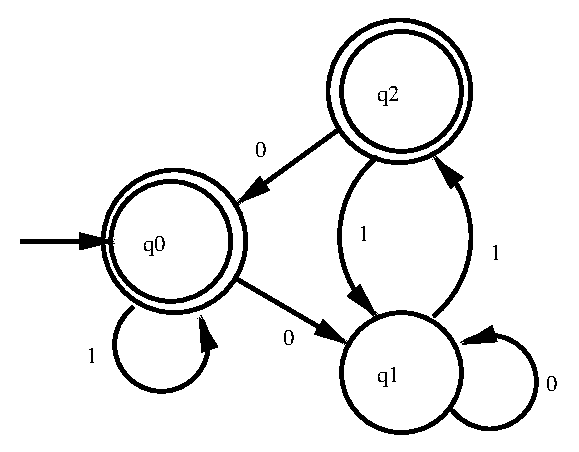
\includegraphics[width=0.35\textwidth]{figs/dfa4.eps}
}
\end{center}
Do so by starting from the equivalent GNFA, then remove the state $q_1$, then the state $q_2$ and finally the state $q_0$.


\newpage
\begin{center}
\textbf{(blank space in case you need it for exercise \ref{conversion})}
\end{center}





\newpage
\section{Non Regular Languages [8 points]}\label{non-regular}
Use the Pumping Lemma to prove that the following languages are not regular.
\begin{enumerate}[label=(\roman*)]
\item $L_1 = \set{www \mid w\in\Sigma^*}$, $\Sigma = \set{0, 1}$.
\item $L_2 = \set{1^{2^n} \mid n\ge 1}$, $\Sigma = \set{1}$.
\end{enumerate}


\newpage
\begin{center}
\textbf{(blank space in case you need it for exercise \ref{non-regular})}
\end{center}




\end{document}
